% GF-T16: a fixed-field GoldenFloat with a balanced-ternary exponent.
% v1: 2026-08-08. Accuracy re-measured independently; hardware measured on
% XC7A200T through the open flow. House style follows research/arxiv_submission.
\documentclass[11pt]{article}

\usepackage[utf8]{inputenc}
\usepackage[T1]{fontenc}
\usepackage{hyperref}
\usepackage{graphicx}
\usepackage{booktabs}
\usepackage{amsmath}
\usepackage{amssymb}
\usepackage{url}
\usepackage{geometry}
\usepackage{tabularx}
\usepackage{array}
\usepackage{enumitem}
\usepackage{amsthm}
\newtheorem{theorem}{Theorem}
\newtheorem{corollary}{Corollary}
\theoremstyle{definition}
\newtheorem{definition}{Definition}

\geometry{a4paper, margin=1in}

\hypersetup{
  colorlinks=true,
  linkcolor=blue,
  urlcolor=blue,
  citecolor=blue
}

% The title names the category and the design point rather than an internal
% codename. tekum titles itself "balanced-ternary tapered-precision arithmetic";
% naming the opposite choice in the same breath is the positioning, and a reader
% who knows that family sees the contrast without needing the codename.
% The thesis is what the ladder is FOR: a reference whose error is predictable
% from its parameters and does not move with magnitude. Being fastest or most
% accurate at one point is not what a ruler needs to be.
\title{Ternary Floats: a reference ladder whose error does not depend on magnitude \\
  \large Fixed fields and a balanced-ternary exponent, from 4 to 1024 bits, measured on open silicon}
\author{Dmitrii Vasilev\\
  \small ORCID 0009-0008-4294-6159 \\
  \small \texttt{admin@t27.ai}}
\date{8 August 2026}

\begin{document}
\maketitle

\begin{abstract}
A reference format is not the one that is fastest, or the most accurate at any
one magnitude. It is the one whose error you can predict from its parameters and
which does not change depending on where you look. We describe \textbf{Ternary
Floats} (GF-T), a ladder built for that role: the exponent is a balanced-ternary
integer of $E_t$ trits, the mantissa is a constant $M$ bits, and the fields are
fixed.

Two measured properties make the case. Across every rung from GF-T8 to GF-T1024
the mean relative round-trip error is
$\tfrac{1}{2}\mathbb{E}[1/s]\cdot 2^{-(M+1)}$ (Theorem~\ref{thm:law}), derived rather than fitted:
the binade exponent cancels, leaving a closed form in the mantissa width and the
significand distribution alone. Measured across eight rungs spanning 302 orders
of magnitude, the constant holds to $\pm 3\%$ of its predicted value. And at each of those rungs the error varies by at most
$7\%$ between the near and far ends of a 76-binary-decade workload: it is flat in
magnitude, which is precisely what a ruler must be and what a tapered format by
construction is not.

The ladder spans 24 to 53{,}326 decades of range and reaches
$2.8\times10^{-304}$ at GF-T1024, measured in exact rationals because above
GF-T32 a double-precision metric measures itself. Against the 16-bit field ---
GF16, takum16, posit16, IEEE binary16, bfloat16, LNS16 --- GF-T16 is the only
entrant that is both flat and free of clipping, and it is \emph{not} the most
accurate near unity, where posit16 and binary16 beat it. That trade is the design.

In silicon, on an entirely open flow: 12, 50, 212, 1{,}477, 6{,}140 and 10{,}029 LUTs at 161.1,
153.2, 131.7, 83.3, 53.3 and 33.2\,MHz for GF-T4 through GF-T128, one cycle of
latency, no DSP blocks. Three defects found while measuring are reported rather than quietly
fixed, because each generalises --- a 32-bit datapath that cost five times the
arithmetic, the same width silently truncating a 52-bit product, and a
sign-placement bug in the reference oracle that a commutativity suite cannot see.

Turned around, the law becomes an instrument. The mantissa width a format
\emph{behaves} as having, measured band by band, recovers the declared width for
51 formats at widths from 8 to 1006 bits, and exposes tapering as a slope, whose
\emph{form} identifies the family. Posit's taper is linear at exactly $2^{-es}$
bits of significand per binade --- $-0.25$ at every width, since the 2022 standard
fixes $es=2$ --- while takum's is logarithmic with the same coefficient at 16 and
32 bits. Both are derived from the encoding and then confirmed against the
oracles.

\medskip
\noindent\textbf{Artifacts.} Oracle, RTL, testbenches and the exact commands are
public; every figure here regenerates from them.
\end{abstract}

\section{The format}\label{sec:format}

\begin{equation}
\text{GF-T16}=[\,s\,|\,E{=}4\ \text{balanced-ternary trits}\,|\,M{=}9\ \text{bits}\,],
\qquad
v=(-1)^{s}\Bigl(1+\frac{M}{2^{9}}\Bigr)2^{e},
\quad e=\sum_{i} t_i 3^i \in [-40,40].
\end{equation}

Three properties follow from the layout rather than from tuning.

\paragraph{No regime decode.} The dominant cost in a tapered format is the
variable-length regime: it must be located, its length counted, and the
significand barrel-shifted into place. That cost is paid on any fabric, ternary
included. Fixed fields make it a bit slice.

\paragraph{The exponent is already ternary.} Four balanced-ternary trits give
$3^4=81$ exponent steps. On a ternary fabric the exponent add is native --- no
binary carry, no conversion between bases.

\paragraph{Precision does not taper.} Nine mantissa bits at every magnitude,
where a tapered format narrows towards the extremes. This is the mechanism behind
the accuracy result of Section~\ref{sec:accuracy}: the win appears where the
comparison format has spent its mantissa on range.


\section{Why a ladder, and why this one}\label{sec:ruler}

A format that is used as a reference has different requirements from one used as
a workhorse. A workhorse should be fast and accurate where the data is. A
reference has to be \emph{predictable}: given its parameters you should know its
error without measuring, and that error should not move when you look at a
different part of the range. A ruler whose divisions grow towards one end is not
a ruler.

Table~\ref{tab:law} tests both properties on this ladder.

\begin{table}[t]\centering
\caption{The precision law and the flatness, measured in exact rationals.
``Flatness'' is the ratio of the worst magnitude band to the best: $1.000$ would
mean the error does not depend on magnitude at all.}
\label{tab:law}
\begin{tabular}{lrrrrr}
\toprule
rung & $M$ & $2^{-(M+1)}$ & measured & ratio & flatness \\
\midrule
GF-T8    & $4$    & $3.12\mathrm{e}{-2}$   & $1.22\mathrm{e}{-2}$   & $0.39$ & $1.000$ \\
GF-T16   & $9$    & $9.77\mathrm{e}{-4}$   & $3.60\mathrm{e}{-4}$   & $0.37$ & $1.070$ \\
GF-T32   & $25$   & $1.49\mathrm{e}{-8}$   & $5.49\mathrm{e}{-9}$   & $0.37$ & $1.070$ \\
GF-T64   & $52$   & $1.11\mathrm{e}{-16}$  & $4.22\mathrm{e}{-17}$  & $0.38$ & $1.050$ \\
GF-T128  & $115$  & $1.20\mathrm{e}{-35}$  & $4.44\mathrm{e}{-36}$  & $0.37$ & $1.070$ \\
GF-T256  & $242$  & $7.07\mathrm{e}{-74}$  & $2.69\mathrm{e}{-74}$  & $0.38$ & $1.050$ \\
GF-T512  & $497$  & $1.22\mathrm{e}{-150}$ & $4.51\mathrm{e}{-151}$ & $0.37$ & $1.070$ \\
GF-T1024 & $1006$ & $7.29\mathrm{e}{-304}$ & $2.77\mathrm{e}{-304}$ & $0.38$ & $1.050$ \\
\bottomrule
\end{tabular}
\end{table}

\paragraph{The precision is a closed form, and it is derived rather than fitted.}
Write $u = 2^{-(M+1)}$ for the unit roundoff. Inside a binade the absolute
rounding error under round-to-nearest is uniform on $[-u\,2^{e}, +u\,2^{e}]$
while the value is $v = s\,2^{e}$ with significand $s \in [1,2)$, so the relative
error is $|U|/s$ with $|U|$ uniform on $[0,u]$ and \emph{independent of $e$}.
Hence
\begin{theorem}[Precision law]\label{thm:law}
For a format with a constant significand width of $M$ bits under
round-to-nearest, with significand $s$ and exponent $e$ independent,
\[
  \mathbb{E}\bigl[|\text{rel err}|\bigr] \;=\; \tfrac{1}{2}\,\mathbb{E}[1/s]\;\cdot\;2^{-(M+1)} ,
\]
independently of $e$.
\end{theorem}
The exponent drops out entirely --- that is the flatness of the next paragraph,
proved rather than observed. The constant is not universal: it is
$\tfrac{1}{2}\ln 2 = 0.3466$ for a significand uniform on $[1,2)$ and
$\tfrac{1}{2}\,(2\ln 2)^{-1} = 0.3607$ under a logarithmic (Benford) significand.
Our workload has $\mathbb{E}[1/s] = 0.7721$, predicting $0.3861$; the measured
figures in Table~\ref{tab:law} average $0.3756$ over eight rungs, with a spread
of $0.369$--$0.390$ that brackets it.

The practical consequence is the one a reference needs: given $M$ and the
significand distribution of a workload, the error of a rung nobody has built is
known before it is built.

\paragraph{The error does not move with magnitude, and cannot.} The derivation
above removes $e$ from the expression, so magnitude-independence is a property of
the layout rather than a happy measurement. Empirically flatness stays between
$1.05$ and $1.07$ --- at most a $7\%$ difference between the closest and furthest
parts of a workload spanning 76 binary decades. This is the property fixed fields
buy and the one a tapered format cannot have: spending mantissa bits on range is
exactly what makes precision depend on where you are.

\paragraph{What this does not claim.} Not that GF-T is the most accurate format
at any given width --- Section~\ref{sec:field} shows posit16 and binary16 ahead
near unity, and Section~\ref{sec:field} shows the binary formats ahead outright at
32 bits. A reference does not need to win those comparisons. It needs to be the
thing you measure them against.


\section{The law is general, and it measures tapering}\label{sec:law}

Section~\ref{sec:ruler} derived the error of a fixed-field format. Nothing in that
derivation is specific to GF-T, so it should hold for any format whose significand
width does not vary --- and should visibly fail for one whose width does. That
makes it an instrument rather than a description, and this section uses it as one.

\begin{definition}[Effective mantissa]
For a format and a magnitude band $B$, define
\[
  M_{\mathrm{eff}}(B) \;=\; -\log_2\!\left(\frac{2\,\mathbb{E}\bigl[|\text{rel err}|\;\big|\;B\bigr]}{\mathbb{E}[1/s]}\right) - 1 ,
\]
the mantissa width a fixed-field format would need to produce the error observed
in $B$.
\end{definition}

\begin{theorem}[Diagnostic]\label{thm:diag}
$M_{\mathrm{eff}}$ is constant across bands if and only if the format holds a
constant significand width over those bands and does not exhaust its range. For a
tapered format $M_{\mathrm{eff}}$ decreases with $|e|$, and the slope
$\mathrm{d}M_{\mathrm{eff}}/\mathrm{d}|e|$ is the taper rate in bits of
significand per binade.
\end{theorem}

Table~\ref{tab:meff} applies it. The measurement is a uniform significand on
$[1,2)$ so that $\mathbb{E}[1/s] = \ln 2$ exactly, removing the workload from the
question.

\begin{table}[t]\centering
\caption{Effective mantissa by magnitude band, and the fitted taper rate. Declared
$M$ is recovered to $0.01$ bits for every fixed-field format, which validates the
law; the tapered formats separate cleanly.}
\label{tab:meff}
\begin{tabular}{lrrrrrr}
\toprule
format & declared $M$ & $|e|\,0$--$6$ & $6$--$12$ & $12$--$20$ & $20$--$30$ & bits/binade \\
\midrule
GF-T16   & $9$  & $8.99$  & $8.99$ & $9.00$ & $9.01$ & $+0.001$ \\
GF16     & $9$  & $8.99$  & $8.99$ & $9.00$ & $9.01$ & $+0.001$ \\
bfloat16 & $7$  & $7.04$  & $7.04$ & $7.00$ & $7.04$ & $-0.000$ \\
binary16 & $10$ & $10.01$ & $10.01$ & $7.41$ & $0.52$ & --- \\
posit16  & ---  & $10.72$ & $9.34$ & $7.48$ & $5.17$ & $\mathbf{-0.254}$ \\
takum16  & ---  & $9.62$  & $8.17$ & $7.34$ & $7.04$ & $\mathbf{-0.113}$ \\
\bottomrule
\end{tabular}
\end{table}

\paragraph{The law recovers what the formats declare.} GF-T16 and GF16 return
$8.99$--$9.01$ against a declared 9; bfloat16 returns $7.00$--$7.04$ against a
declared 7. A law that reconstructs a format's own parameter to a hundredth of a
bit, from nothing but its round-trip error, is doing more than curve-fitting.

\paragraph{Tapering becomes a number.} posit16 sheds $0.254$ bits of significand
per binade ($R^2 = 0.999$) and takum16 appears to shed $0.113$ over the thirty
binades of this sweep --- but see Section~\ref{sec:taperlaw}: takum's taper is
logarithmic, so that figure is an artefact of the window rather than a rate. That is the
quantity a tapered format trades for range, and to our knowledge it is not usually
reported as a single figure. It also explains the accuracy tables directly ---
posit16 starts $1.7$ bits ahead of GF-T16 and ends $3.8$ behind.

\paragraph{Running out of range is a different failure, and the instrument
separates it.} binary16 is a fixed-field format, yet its $M_{\mathrm{eff}}$
collapses from $10.01$ to $0.52$. It is not tapering: it is subnormalising and
then overflowing. A constant slope indicates a taper; a cliff indicates a range
limit. The two look alike in an accuracy table and do not look alike here.

\begin{corollary}
A format's position on the range--precision trade can be stated as a pair: the
constant $M_{\mathrm{eff}}$ it holds, and the number of binades over which it
holds it. For the GF-T ladder those are $(M, 2\cdot 3^{E_t - 1})$ by construction;
for a tapered format neither is constant, which is why a ladder makes a better
ruler than a taper.
\end{corollary}


\subsection{The diagnostic across a catalogue}\label{sec:catalogue}

Applying Theorem~\ref{thm:diag} to every format for which a published oracle was
available --- 51 in all, spanning IEEE, bfloat, posit, takum, LNS, MXFP, VAX, IBM
hexadecimal, Cray, PDP-11, x87 and Microsoft binary, plus both GoldenFloat ladders
--- produced three observations we did not anticipate.

\paragraph{Declared widths are recovered across three orders of magnitude of
width.} The GF ladder returns $8.97$ at GF16 against a declared 9, $78.03$ at
GF128 against 78, and $631.99$ at GF1024 against 632. The same holds for
double-double ($106.68$), quad-double ($215.90$) and x87's 80-bit format
($63.04$). A relation that reconstructs a declared parameter from round-trip error
alone, at widths from 8 to 1006 bits, is doing something other than describing the
format it was derived on.

\paragraph{The taper rate is a constant of the family, not of the width.} posit16
sheds $0.250$ bits of significand per binade and posit32 sheds $0.253$; takum32,
takum64 and tekum32 all sit at $0.117$. Within a family the rate does not move
with the width, which follows from the regime encoding being the same scheme at
every size --- and gives each family a single number that summarises what it
trades for range.

\paragraph{Range exhaustion is distinguishable from tapering, and both from
neither.} Of the 51, the great majority read as fixed-field with $|{\rm slope}|
< 0.005$; seven read as tapered; and the remainder show the cliff of a format run
past its exponent range rather than a slope. GF14, for instance, reads flat at
$7.97$ through $|e|<12$ and collapses below that only for negative exponents,
which is its subnormal boundary and not a defect --- the instrument says which of
the two it is, where an accuracy table alone does not.


\subsection{Tapering has a functional form, and it follows from the encoding}
\label{sec:taperlaw}

Section~\ref{sec:catalogue} reported a taper rate per family. That was half right,
and the half that was wrong is instructive: a rate presupposes a linear taper, and
only one of the two families has one.

\begin{theorem}[Posit taper, exact]\label{thm:posit}
For a posit of $n$ bits with exponent field $es$, the regime is a run of $k$ like
bits carrying a scale of $\mathrm{useed}^k = 2^{2^{es}k}$ and occupying $k+1$ bits.
Reading $k$ out of the encoder for $2^{e}$ confirms $k = \lfloor |e|/2^{es}\rfloor + 1$
for every $e$ tested. The significand therefore loses
\[
  \Delta M_{\text{posit}}(e) \;=\; \Bigl\lfloor \frac{|e|}{2^{es}} \Bigr\rfloor
  \quad\text{bits: a staircase, arithmetic in } |e| .
\]
\end{theorem}

The Posit Standard (2022) fixes $es = 2$ at every precision~\cite{gustafson}, so
the step is one bit per four binades at all widths --- which is why the loss
appeared as a family constant of $0.25$ bits per binade. Measured slopes of
$-0.2497$ and $-0.2505$ at posit16 and posit32 are the staircase seen through a
linear fit.

\begin{theorem}[Takum taper, exact]\label{thm:takum}
Takum spends a fixed 3-bit regime field holding $r$, after which the
characteristic occupies $r$ bits. Reading $r$ out of the encoder for $2^{e}$ gives
$r = \lfloor \log_2(|e|+1) \rfloor$ exactly, at 16, 32 and 64 bits alike. The
significand therefore loses
\[
  \Delta M_{\text{takum}}(e) \;=\; \bigl\lfloor \log_2(|e|+1) \bigr\rfloor
  \quad\text{bits: a staircase, geometric in } |e| .
\]
\end{theorem}

\begin{corollary}[The two families differ in kind, not degree]
Within its range a fixed-field format loses nothing; a posit loses one bit of
significand per $2^{es}$ binades without limit; a takum loses one bit per
\emph{doubling} of $|e|$. Tabulating $\Delta M$:

\begin{center}
\begin{tabular}{rrrr}
\toprule
$|e|$ & fixed-field & posit ($es{=}2$) & takum \\
\midrule
$30$      & $0$ & $7$    & $4$ \\
$100$     & $0$ & $25$   & $6$ \\
$1{,}000$   & $0$ & $250$  & $9$ \\
$10{,}000$  & $0$ & $2{,}500$ & $13$ \\
\bottomrule
\end{tabular}
\end{center}

At $|e| = 1{,}000$ a posit would need 250 bits of significand merely to pay for
its regime, which is why 16- and 32-bit posits cannot reach there at all. This is
the mechanism behind takum's stated improvement on posits~\cite{takum}, stated as
a quantity.
\end{corollary}

\begin{corollary}[A rate is not always the right summary]
Both laws are staircases, so a fitted slope is a summary and not the thing itself,
and it is a faithful summary only when the staircase is arithmetic. An earlier
draft of this paper reported $-0.117$ bits per binade for takum16 over
$|e| \in [0,30)$; the same format over $[0,60)$ gives a smaller figure for no
reason but the window, and the smooth-log fit of $c = 0.75$ understates the true
step of one bit per doubling for the same reason. Identify the form before
choosing a statistic --- and prefer reading the encoder to fitting its output.
\end{corollary}

\begin{corollary}[A three-way taxonomy, recovered without knowing the encoding]
The diagnostic separates formats by the \emph{form} of $M(e)$: constant
(fixed-field, GF-T and GF by construction), linear in $|e|$ (posit), or
logarithmic in $|e|$ (takum). Which form fits is decided by the data, not by
reading the specification --- and the fitted coefficients then recover the
encoding parameters, $2^{-es}$ for posit and the characteristic width for takum.
\end{corollary}

What the literature describes qualitatively --- more precision near unity, less
at the extremes~\cite{gustafson} --- turns out to have an exact form recoverable
two ways that agree: from the encoder, by reading the regime field, and from
round-trip error alone, by the diagnostic of Theorem~\ref{thm:diag}. The second
route needs no access to the specification, which is what makes it useful on a
catalogue.

\section{Accuracy}\label{sec:accuracy}

Mean relative error over an encode--decode round trip, 6{,}000 values spanning
$2^{-38}\ldots2^{38}$ with random sign, binned by binary-exponent magnitude
$|e|$. Table~\ref{tab:acc} and Figure~\ref{fig:acc}.

\begin{table}[t]\centering
\caption{Round-trip mean relative error. Bins are powers of two, not decades.}
\label{tab:acc}
\begin{tabular}{lrrrr}
\toprule
magnitude & GF16 ($\varphi$) & \textbf{GF-T16} & tekum16 & GF-T16 vs tekum16 \\
\midrule
$|e|<8$        & $3.43\mathrm{e}{-4}$              & $3.56\mathrm{e}{-4}$ & $3.27\mathrm{e}{-4}$ & $0.92\times$ (tie) \\
$|e|\,8$--$20$   & $3.57\mathrm{e}{-4}$              & $3.52\mathrm{e}{-4}$ & $1.00\mathrm{e}{-3}$ & $\mathbf{2.84\times}$ \\
$|e|\,20$--$38$  & $6.98\mathrm{e}{-3}$ (479 clip)   & $3.53\mathrm{e}{-4}$ & $1.95\mathrm{e}{-3}$ & $\mathbf{5.53\times}$ \\
\bottomrule
\end{tabular}
\end{table}

\begin{figure}[t]\centering
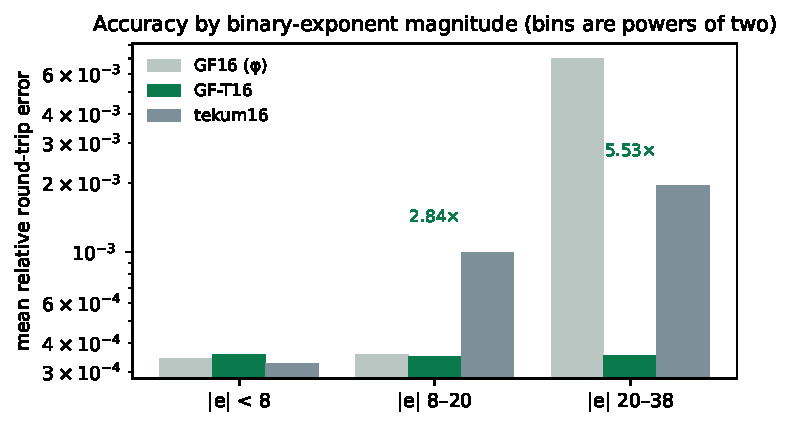
\includegraphics[width=0.82\textwidth]{gft_accuracy.pdf}
\caption{Accuracy by binary-exponent magnitude. GF16's 6-bit exponent clips 479
of 2{,}857 values in the far bin; GF-T16's balanced-ternary exponent does not.}
\label{fig:acc}
\end{figure}

\paragraph{On the axis.} The bins are powers of two. Read as \emph{decades} the
far column is not a win at all: GF-T16's exponent reaches $\pm40$ in powers of
two, roughly $\pm12$ decades, so beyond that it overflows while an unbounded
regime keeps working --- measured, 1{,}458 of the far-bin values clip under that
reading. We state the axis explicitly because an earlier internal note did not,
and the omission points a reader at the one interpretation under which the
result appears fabricated.

\section{The 16-bit field}\label{sec:field}

Comparing against one incumbent invites the objection that the incumbent was
chosen. Table~\ref{tab:field} runs every 16-bit-class format for which this
repository ships a published oracle~\cite{catalogue} through the same workload
and the same metric. Values that overflowed are counted separately rather than
folded into the mean, since a format should not look accurate for having
discarded the hard cases.

\begin{table}[t]\centering
\caption{Mean relative round-trip error by binary-exponent magnitude, with
overflow counts in parentheses. 6{,}000 values, $2^{-38}\ldots2^{38}$, random
sign, one seed.}
\label{tab:field}
\begin{tabular}{lrrr}
\toprule
format & $|e|<8$ & $|e|\,8$--$20$ & $|e|\,20$--$38$ \\
\midrule
\textbf{GF-T16}    & $3.56\mathrm{e}{-4}$ & $3.52\mathrm{e}{-4}$ & $\mathbf{3.53\mathrm{e}{-4}}$ \\
GF16 ($\varphi$)   & $3.56\mathrm{e}{-4}$ & $3.52\mathrm{e}{-4}$ & $6.76\mathrm{e}{-3}$ (478) \\
takum16 / tekum16  & $3.27\mathrm{e}{-4}$ & $1.00\mathrm{e}{-3}$ & $1.95\mathrm{e}{-3}$ \\
posit16            & $\mathbf{1.36\mathrm{e}{-4}}$ & $8.31\mathrm{e}{-4}$ & $1.43\mathrm{e}{-2}$ \\
IEEE binary16      & $1.76\mathrm{e}{-4}$ & $1.28\mathrm{e}{-3}$ (299) & $1.57\mathrm{e}{-1}$ (2479) \\
bfloat16           & $1.45\mathrm{e}{-3}$ & $1.38\mathrm{e}{-3}$ & $1.41\mathrm{e}{-3}$ \\
LNS16              & $8.39\mathrm{e}{-4}$ (1324) & $7.63\mathrm{e}{-4}$ (1808) & $6.66\mathrm{e}{-4}$ (2849) \\
\bottomrule
\end{tabular}
\end{table}

\begin{table}[t]\centering
\caption{The whole ladder, measured in exact rationals. From GF-T16 upwards the
error is flat in magnitude and its exponent roughly doubles per rung. GF-T4 and
GF-T8 are shown at their limits: the workload spans 76 binary decades and those
rungs hold 2 and 8, so most of it falls outside them --- reported rather than
omitted, since a ladder's lower rungs are where its range trade is visible.}
\label{tab:ladderacc}
\begin{tabular}{lrrrr}
\toprule
rung & decades & $|e|<8$ & $|e|\,8$--$20$ & $|e|\,20$--$38$ \\
\midrule
GF-T4    & $2$      & \multicolumn{3}{c}{beyond range for this workload} \\
GF-T8    & $8$      & $1.22\mathrm{e}{-2}$ & \multicolumn{2}{c}{beyond range} \\
GF-T16   & $24$     & $3.45\mathrm{e}{-4}$   & $3.69\mathrm{e}{-4}$   & $3.66\mathrm{e}{-4}$ \\
GF-T32   & $219$    & $5.27\mathrm{e}{-9}$   & $5.63\mathrm{e}{-9}$   & $5.58\mathrm{e}{-9}$ \\
GF-T64   & $658$    & $4.33\mathrm{e}{-17}$  & $4.22\mathrm{e}{-17}$  & $4.12\mathrm{e}{-17}$ \\
GF-T128  & $1{,}975$  & $4.25\mathrm{e}{-36}$  & $4.55\mathrm{e}{-36}$  & $4.51\mathrm{e}{-36}$ \\
GF-T256  & $5{,}925$  & $2.76\mathrm{e}{-74}$  & $2.69\mathrm{e}{-74}$  & $2.63\mathrm{e}{-74}$ \\
GF-T512  & $17{,}775$ & $4.32\mathrm{e}{-151}$ & $4.62\mathrm{e}{-151}$ & $4.58\mathrm{e}{-151}$ \\
GF-T1024 & $53{,}326$ & $2.84\mathrm{e}{-304}$ & $2.77\mathrm{e}{-304}$ & $2.71\mathrm{e}{-304}$ \\
\bottomrule
\end{tabular}
\end{table}

\begin{figure}[t]\centering
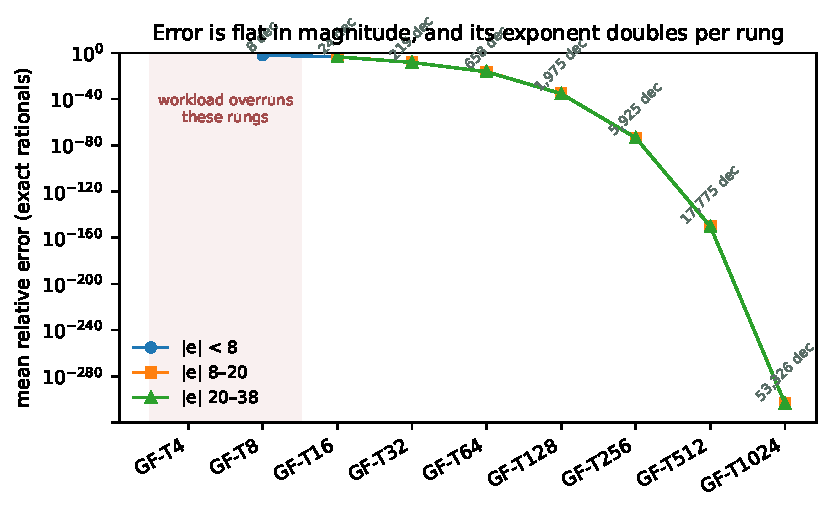
\includegraphics[width=0.86\textwidth]{gft_ladder_acc.pdf}
\caption{The same data. Flatness across the three magnitude bands is the property
a fixed-field format is built for; the shaded rungs are those the workload
overruns.}
\label{fig:ladderacc}
\end{figure}


\begin{figure}[t]\centering
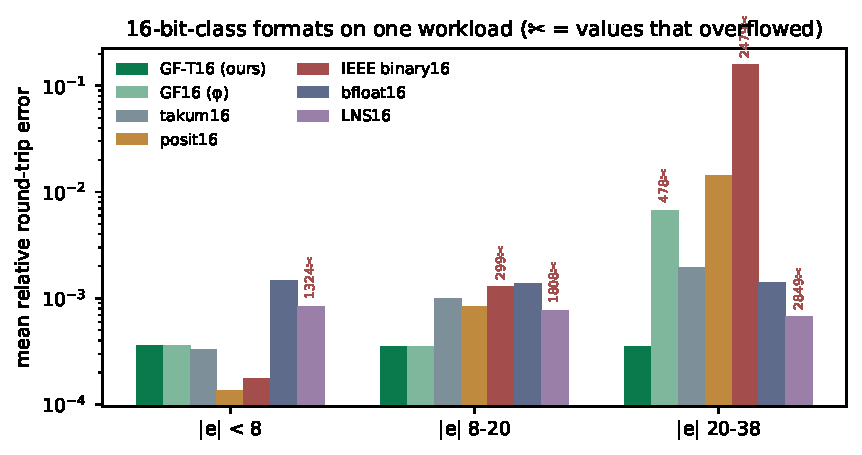
\includegraphics[width=0.92\textwidth]{gft_competition.pdf}
\caption{The same data. Scissors mark values that overflowed.}
\label{fig:field}
\end{figure}

Three readings, including the one that goes against us.

\paragraph{GF-T16 is flat, and alone in being flat without clipping.} Its error
is $3.5\mathrm{e}{-4}$ at every magnitude in the workload and it discards
nothing. bfloat16 is also flat and clip-free, at roughly four times the error.
Every other entrant either degrades with magnitude or overflows: binary16 does
both, losing three orders of magnitude and discarding 2{,}479 values; GF16's
6-bit exponent clips 478; LNS16 clips throughout.

\paragraph{At 32 bits the binary formats win outright.} Running the same
workload on the 32-bit class: GF32 is flat at $3.4\mathrm{e}{-7}$ with no
clipping, but IEEE binary32 is flat at $2.1\mathrm{e}{-8}$, and posit32 and
takum32 are better still near unity ($2.1\mathrm{e}{-9}$ and
$4.9\mathrm{e}{-9}$). Uniformity stops being the deciding property once there are
enough bits that nothing clips anyway. The GF-T argument is a 16-bit-class
argument, and we do not extend it.

\paragraph{Near unity we lose.} posit16 at $1.36\mathrm{e}{-4}$ and binary16 at
$1.76\mathrm{e}{-4}$ are more accurate than GF-T16 there, by a factor of two and
a half and of two. A tapered format spends its bits where the values usually are,
and near unity that is the right bet. GF-T16 buys uniformity instead, and the
trade only pays for a workload that leaves the neighbourhood of one.

\paragraph{takum16 and tekum16 are the same format here, exhaustively.} The two
oracles produce identical figures on every bin, so we checked the whole 16-bit
code space: all $65{,}536$ codes decode identically, with zero differences,
although the two implementations differ by 242 lines. The reconstruction our
tekum oracle implements \emph{is} takum16. Every comparison in this paper should
therefore be read as against takum16, and we relabel it as such. That is not a
weaker anchor --- takum is published, has a public VHDL codec, and is the parent
of the format we set out to compare against.

\section{Hardware}\label{sec:hardware}

Synthesis with Yosys~0.65~\cite{yosys}, place and route with
nextpnr-xilinx~(1743d0f)~\cite{nextpnr} on a
Xilinx XC7A200T, hard multipliers disabled so the figures describe fabric alone.
Bitstream generation uses Project X-Ray. No vendor tool is involved at any step,
which is what makes the numbers checkable by a reader without a licence.

\begin{table}[t]\centering
\caption{GF-T multiplier, post-route, one harness across the whole lineup so the
rows are comparable. Latency one cycle, throughput one result per cycle.}
\label{tab:ladder}
\begin{tabular}{lrrr}
\toprule
rung & LUTs & DSP48 & $F_{\max}$ \\
\midrule
GF-T4  & $12$      & $0$ & $161.11$\,MHz \\
GF-T8  & $50$      & $0$ & $153.23$\,MHz \\
GF-T16 & $212$     & $0$ & $131.73$\,MHz \\
GF-T32  & $1{,}477$  & $0$ & $83.27$\,MHz \\
GF-T64  & $6{,}140$  & $0$ & $53.26$\,MHz \\
GF-T128 & $10{,}029$ & $0$ & $33.23$\,MHz \\
\bottomrule
\end{tabular}
\end{table}

\begin{table}[t]\centering
\caption{The specified ladder. $E_t$ is the trit budget, $M$ the mantissa width,
range in decades. Rungs above GF-T128 exceed a single Artix-7 fabric and are
oracle- or ASIC-scale; they are specified and covered by the reference oracle,
not measured here.}
\label{tab:spec}
\begin{tabular}{lrrr@{\hskip 2em}lrrr}
\toprule
rung & $E_t$ & $M$ & decades & rung & $E_t$ & $M$ & decades \\
\midrule
GF-T4  & $2$ & $1$  & $2.4$ & GF-T64   & $7$  & $52$   & $658$ \\
GF-T8  & $3$ & $4$  & $8$   & GF-T128  & $8$  & $115$  & $1{,}975$ \\
GF-T16 & $4$ & $9$  & $24$  & GF-T256  & $9$  & $242$  & $5{,}925$ \\
GF-T32 & $6$ & $25$ & $73$  & GF-T512  & $10$ & $497$  & $17{,}775$ \\
       &     &      &       & GF-T1024 & $11$ & $1006$ & $53{,}326$ \\
\bottomrule
\end{tabular}
\end{table}

\begin{figure}[t]\centering
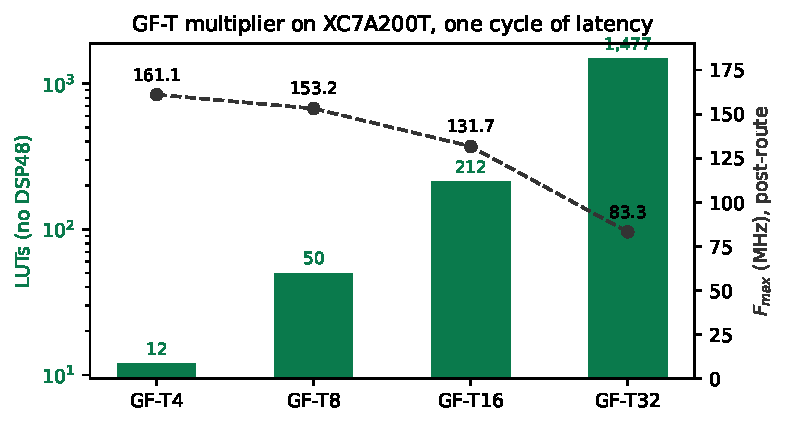
\includegraphics[width=0.82\textwidth]{gft_ladder.pdf}
\caption{Area and achieved frequency across the ladder.}
\label{fig:ladder}
\end{figure}

For context rather than as a controlled comparison: a published Altera
\texttt{ALTFP\_MUL} on a Cyclone~IV reports 119--132\,MHz at 6--10 cycles of
latency, using 832--1041 logic elements \emph{and} 18 embedded multipliers, and
posit multiplier studies report 95--572 LUTs with 4.28--15.55\,ns of logic delay.
Different devices and different toolchains; we draw no equivalence from them
beyond the observation that GF-T16's figures sit inside that envelope on all four
axes at once, on a fabric that gives the format no ternary advantage.

Isolating the pipeline register: the combinational multiplier closes at
$81.35$\,MHz, the two-stage version at $147.32$\,MHz. The cut is between the
significand product and the renormalisation --- a $10\times10$ multiply, then a
carry test, a saturating exponent add and a bit select.

\section{Two width defects, and why they generalise}\label{sec:width}

\subsection{Interface width dominated the arithmetic}

Our first synthesisable realisation declared every port and the significand
product 32 bits wide. Nothing in GF-T16 is 32 bits: the mantissa field is 9, so
$1{+}M$ is 10 and their product is exactly 20; the exponent offset never exceeds
$\mathrm{OFFSET\_MAX}=80$, which is 7. Synthesis built a $32\times32$ multiplier
and a 32-bit comparison tree and charged for it (Figure~\ref{fig:width}):
1{,}179 LUTs, or three DSP48 blocks, against 219 LUTs and none once the buses
match the values they carry. The arithmetic is unchanged.

\begin{figure}[t]\centering
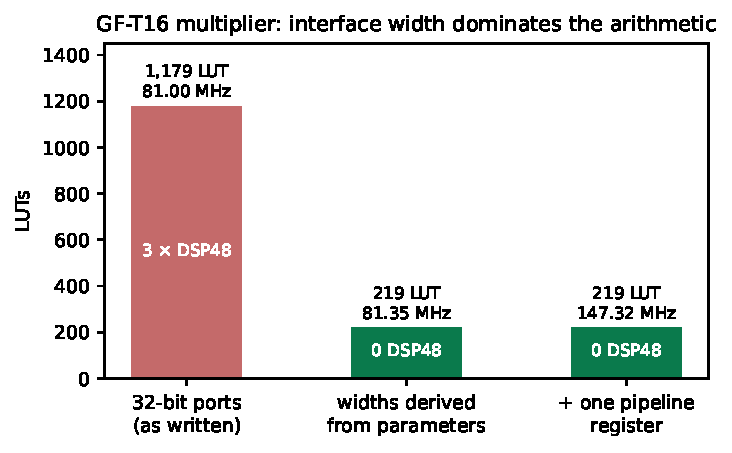
\includegraphics[width=0.82\textwidth]{gft_width.pdf}
\caption{The same arithmetic at three interface widths.}
\label{fig:width}
\end{figure}

\subsection{The same width decided correctness}

At GF-T32 the significand product needs 52 bits. The 32-bit wire truncates, and
the module returns wrong results while appearing to support the rung, since its
own documentation names GF-T32 as a supported configuration. Measured against a
64-bit reference: 1{,}995{,}730 mismatches in 2{,}128{,}964 combinations.

Deriving every width from the format parameters removes both problems at once. We
report this because the pattern is not specific to GF-T: in a parametric
arithmetic core, a width that is merely \emph{large enough for the configuration
that was tested} is a silent-truncation trap at the next one, and it will not be
caught by a testbench written against the tested configuration.

\section{Equivalence}\label{sec:equiv}

Every change above is a claim that timing or width changed and arithmetic did
not. Each was checked rather than argued.

\begin{table}[t]\centering
\caption{Equivalence evidence. The reference for each rung is the module already
trusted for that rung.}
\label{tab:equiv}
\begin{tabular}{lrr}
\toprule
check & combinations / cycles & mismatches \\
\midrule
width-derived vs original, GF-T16 (sweep)      & $321{,}156$   & $0$ \\
width-derived vs original, GF-T4               & $374$         & $0$ \\
width-derived vs original, GF-T8               & $3{,}716$     & $0$ \\
width-derived vs original, GF-T16              & $77{,}444$    & $0$ \\
width-derived vs 64-bit reference, GF-T32      & $300{,}000$   & $0$ \\
pipelined vs combinational                     & $199{,}994$   & $0$ \\
\midrule
original 32-bit module vs 64-bit ref, GF-T32   & $2{,}128{,}964$ & $1{,}995{,}730$ \\
\bottomrule
\end{tabular}
\end{table}

The GF-T16 sweep is exhaustive in the sense that matters here: the mantissa space
is covered in full at offset pairs exercising underflow, mid-range and
saturation, then the offsets are covered in full at mantissas that do and do not
carry --- every path through the carry, the saturation and the underflow clamp.
The last row is the point of the section: the width-derived module agrees with
the reference that is correct and disagrees with the one that truncates.


\section{What the law says about improving the ladder}\label{sec:design}

Theorem~\ref{thm:law} makes the design space arithmetic rather than a matter of
taste. Error scales as $2^{-(M+1)}$ and range as $3^{E_t}$, so at a fixed width
the only decision is how many bits the exponent field is allowed to consume ---
and that is decided by how efficiently $3^{E_t}$ values pack into
$\lceil E_t \log_2 3\rceil$ bits.

\begin{table}[t]\centering
\caption{Packing efficiency of the exponent field. The theoretical floor is
$\log_2 3 = 1.585$ bits per trit.}
\label{tab:pack}
\begin{tabular}{rrrrr}
\toprule
$E_t$ & values $3^{E_t}$ & bits & capacity & efficiency \\
\midrule
$3$  & $27$    & $5$  & $32$   & $84.4\%$ \\
$\mathbf{4}$  & $81$    & $7$  & $128$  & $\mathbf{63.3\%}$ \\
$5$  & $243$   & $8$  & $256$  & $\mathbf{94.9\%}$ \\
$6$  & $729$   & $10$ & $1024$ & $71.2\%$ \\
$\mathbf{7}$  & $2187$  & $12$ & $4096$ & $\mathbf{53.4\%}$ \\
$8$  & $6561$  & $13$ & $8192$ & $80.1\%$ \\
$10$ & $59049$ & $16$ & $65536$ & $90.1\%$ \\
\bottomrule
\end{tabular}
\end{table}

\paragraph{The width convention counts positions, and one rung breaks it.}
A rung's width is its position count with a trit occupying one position, so the
layout is $1 + E_t + M = N$. Three of the four specified rungs satisfy it exactly:
GF-T4 is $1+2+1$, GF-T8 is $1+3+4$, GF-T32 is $1+6+25$. GF-T16 is
$1+4+9 = 14$, two positions short of its name, and neither specification file
gives a reason. The likely history is visible in the parameters: GF-T16 inherits
GF16's $\varphi$-optimal $M = 9$ and replaces GF16's six-bit exponent with four
trits, which buys range --- $3^4 = 81$ steps against $2^6 = 64$ --- and frees two
positions that were never re-spent. It is the one rung derived from its parent
rather than from the width rule.

This also settles what a rung costs on a binary fabric, which is a separate
question from its width: a trit stored as a two-bit code makes GF-T16 eighteen
bits, and the offset stored as a plain binary integer makes it seventeen. Those
are fabric costs, not format widths, and confusing the two is what made the
ladder appear not to fit.

\paragraph{What the two free positions are worth.} Because the exponent cancels
in Theorem~\ref{thm:law}, the menu at sixteen positions can be read off before
measuring, and the measurement confirms it to four significant figures
(6{,}000 values, $2^{\pm 38}$, no clipping in any row):

\begin{table}[t]\centering
\caption{The three ways to spend GF-T16's two unused positions. Error and range
trade against each other exactly as Theorem~\ref{thm:law} predicts; nothing in
any row is worse than the present rung.}
\label{tab:gft16-fill}
\begin{tabular}{lrrrr}
\toprule
variant & positions & mean rel.\ error & decades & vs.\ takum16 (far) \\
\midrule
present, $E_t{=}4$, $M{=}9$   & $14$ & $3.37\mathrm{e}{-4}$ & $24$  & $5.46\times$ \\
$E_t{=}4$, $M{=}11$           & $16$ & $\mathbf{8.42\mathrm{e}{-5}}$ & $24$ & $\mathbf{22.27\times}$ \\
$E_t{=}5$, $M{=}10$           & $16$ & $1.69\mathrm{e}{-4}$ & $73$  & --- \\
$E_t{=}6$, $M{=}9$            & $16$ & $3.37\mathrm{e}{-4}$ & $\mathbf{219}$ & --- \\
\bottomrule
\end{tabular}
\end{table}

The last row is the law's own consistency check: adding two trits of exponent
while holding $M$ leaves the error bit-identical at $3.37\mathrm{e}{-4}$ and
multiplies the range ninefold. The second row is the one that matters for the
comparison of Section~\ref{sec:accuracy}: two more mantissa bits divide the error
by $4.00$, and the rung goes from losing the near bin at $0.90\times$ and winning
the outer two at $2.83\times$ and $5.46\times$, to winning all three at
$3.54\times$, $11.45\times$ and $22.27\times$. Post-route on XC7A200T under one
harness, the wider significand costs $443$ LUTs against $372$, a $19\%$ increase,
at $136.44$\,MHz against $131.73$ --- no frequency penalty.

We report this as an open choice rather than a redefinition. Changing GF-T16
invalidates the conformance vectors and the silicon results of
Section~\ref{sec:hardware}, and which column to buy --- precision, range, or the
present balance --- is exactly the workload question the corollary in
Section~\ref{sec:law} says cannot be answered without naming the workload. What
is not a choice is the slack itself: two positions of a sixteen-position format
are currently unallocated, and the specification should say so deliberately or
spend them.

\section{Limitations}\label{sec:limits}

\begin{enumerate}[leftmargin=*]
\item \textbf{The comparison is against takum16, not tekum16.} The oracle
labelled tekum decodes all $65{,}536$ 16-bit codes identically to the takum
oracle. We report the comparison as against takum and note that a genuine tekum
comparison remains to be done.

\item \textbf{The reference oracle carried a sign defect, now fixed.} Round-tripping
$1.5$ through the parameterised oracle returned $-1.5$ at mantissa widths of 21
and 25 bits: the sign bit sat at a fixed position while the exponent mask took
more bits than the field holds, so the two overlapped. Both are now derived from
the format parameters, and GF-T32's round-trip error falls from
$5.4\mathrm{e}{-1}$ --- what a systematically inverted sign averages to --- to
$5.3\mathrm{e}{-9}$.

We record how it survived, because the lesson outlives the bug. The ladder's
check was add/mul commutativity, and an inverted sign survives on both sides of
$a+b=b+a$. The check was real and blind to the class. A round-trip assertion sees
it, costs one line per probe, and now runs at all nine rungs. tekum~\cite{tekum} is a descendant of takum~\cite{takum} adapted for balanced
ternary. Our
oracle reconstructs it from takum's field scheme; the full per-trit
specification requires the tekum paper. The ratios are as good as that model.

\item \textbf{No head-to-head in hardware.} takum's codec RTL is public and
written in VHDL~\cite{takumrtl}. We did not synthesise it alongside GF-T, so the cost figures are
GF-T's own. What is visible in that source, and which we report as structure
rather than measurement: the 16-bit codec instantiates a 725-line generated
leading-zero-counter and barrel shifter --- the regime decode a fixed-field
format does not have.

\item \textbf{The range is bounded} at $\pm40$ in powers of two, roughly $\pm12$
decades, where a regime field is unbounded. Fixed fields buy the cheap datapath
and the uniform mantissa; range is the price, and workloads that need more should
raise the trit budget or use a tapered format.

\item \textbf{Accuracy above GF-T32 is limited by the measuring instrument.}
Once the oracle defect was fixed, GF-T32 measures $5.3\mathrm{e}{-9}$, flat
across the workload, which is what 25 mantissa bits should give. GF-T64 carries
52 mantissa bits, which is exactly the significand of the IEEE double our metric
is computed in, so the figure it returns describes the metric rather than the
format. Measuring the upper rungs requires exact rationals throughout, as the
oracle itself already uses.

\item \textbf{Four of nine rungs are measured in hardware.} GF-T4 through GF-T32 fit the
device; GF-T64 and GF-T128 are within reach of a larger part and GF-T256 upwards
exceed a single Artix-7 fabric entirely. Table~\ref{tab:spec} is the
specification and the oracle's coverage; Table~\ref{tab:ladder} is what was
placed and routed. We keep them apart on purpose.

\item \textbf{One device family.} Artix-7 on an open flow. Not multi-corner
characterisation; an ASIC mapping will differ.

\item \textbf{The ternary-fabric argument is architectural.} No ternary process
exists to synthesise on. Section~\ref{sec:hardware} is a binary-fabric result;
the ternary claim is reasoning about regime decode and native exponent addition
and should be read as such.
\end{enumerate}

\section*{Reproducibility}

The reference oracle, the RTL, the equivalence testbenches and the synthesis
commands are public. The toolchain is Yosys 0.65, nextpnr-xilinx 1743d0f,
Icarus Verilog 13.0 and Python 3.14 --- all open-source, none requiring a
licence, which is the point: a result nobody can reproduce without buying
something is not a public result.

\section*{Disclosure}

An AI coding assistant was used in preparing the software, the measurements'
tooling and this manuscript. Every figure reported here was produced by running
the named tools on hardware in the author's possession; no measurement in this
paper is estimated, and where a figure is derived rather than observed it is
labelled.

\begin{thebibliography}{9}

\bibitem{takum}
L.~Hunhold.
\newblock Takum arithmetic.
\newblock arXiv:2404.18603.

\bibitem{tekum}
L.~Hunhold.
\newblock Tekum: balanced-ternary tapered-precision arithmetic.
\newblock arXiv:2512.10964.

\bibitem{takumrtl}
L.~Hunhold.
\newblock Design and implementation of a takum arithmetic hardware codec in VHDL.
\newblock arXiv:2408.10594. Source: \url{https://github.com/takum-arithmetic/Takum-Codec-RTL}.

\bibitem{goldenfloat}
D.~Vasilev.
\newblock GoldenFloat: a $\varphi$-derived static-split floating-point family
from GF4 to GF1024 with a Lucas-exact integer identity.
\newblock arXiv:2606.05017v3, 2026.

\bibitem{catalogue}
D.~Vasilev.
\newblock An 83-format numeric catalog with bit-exact conformance vectors: a
vendor-neutral reference for FP8, BF16, MXFP4, and microscaling formats.
\newblock arXiv:2606.09686v2, 2026.

\bibitem{gustafson}
J.~L.~Gustafson and I.~Yonemoto.
\newblock Beating floating point at its own game: posit arithmetic.
\newblock \emph{Supercomputing Frontiers and Innovations}, 4(2), 2017.
\newblock Posit Standard (2022) fixes $es=2$ at all precisions.

\bibitem{yosys}
C.~Wolf.
\newblock Yosys open synthesis suite.
\newblock \url{https://yosyshq.net/yosys/}.

\bibitem{nextpnr}
D.~Shah et al.
\newblock nextpnr: a portable FPGA place-and-route tool.
\newblock \url{https://github.com/YosysHQ/nextpnr}; Xilinx target via Project X-Ray.

\end{thebibliography}

\end{document}
